%!TEX root = ../main.tex
% Chapter 11: Theoretical Aspects --- Generalization, Expressivity
\chapter{Theoretical Aspects --- Generalization, Expressivity}
\label{ch:theory}

\noindent\textit{This chapter explores the theoretical foundations of deep learning:
why do overparameterized networks generalize? What is their expressive
power? How does the geometry of the loss landscape influence optimization?
We present the PAC framework, VC dimension, Rademacher complexity, the
neural tangent kernel (NTK) theory, and recent results on double descent
and scaling laws.}\medskip

% ============================================================
\section{PAC Framework for Neural Networks}
\label{sec:pac-learning}
\index{PAC learning}

\subsection{Fundamental Definitions}

\begin{definition}[PAC Learning]
\label{def:pac}
A hypothesis class $\mathcal{H}$ is \emph{PAC-learnable} if there exists
an algorithm $\mathcal{A}$ such that, for all $\varepsilon > 0$, $\delta > 0$
and every distribution $\mathcal{D}$ over $\mathcal{X} \times \mathcal{Y}$,
with probability at least $1 - \delta$ over a sample
$S \sim \mathcal{D}^m$:
\begin{equation}
R(h_S) \leq \min_{h \in \mathcal{H}} R(h) + \varepsilon
\end{equation}
as soon as $m \geq m_{\mathcal{H}}(\varepsilon, \delta)$, where
$R(h) = \E_{(x,y) \sim \mathcal{D}}[\ell(h(x), y)]$ is the true risk.
\end{definition}

\begin{theorem}[PAC Generalization Bound]
\label{thm:pac-bound}
For a finite class $\mathcal{H}$, with probability $\geq 1 - \delta$:
\begin{equation}
R(h_S) \leq \hat{R}_S(h_S) + \sqrt{\frac{\log|\mathcal{H}| + \log(1/\delta)}{2m}}
\end{equation}
where $\hat{R}_S$ is the empirical risk.
\end{theorem}

\begin{remark}
This bound is too coarse for modern neural networks
that have billions of parameters ($\log|\mathcal{H}|$ would be enormous).
Finer complexity measures are needed.
\end{remark}

% ============================================================
\section{VC Dimension of Neural Networks}
\label{sec:vc-dimension}
\index{VC dimension}

\begin{definition}[VC Dimension]
\label{def:vc-dim}
The Vapnik-Chervonenkis dimension of $\mathcal{H}$ is the maximum size
of a point set that $\mathcal{H}$ can \emph{shatter},
i.e., realize all $2^m$ possible dichotomies.
\end{definition}

\begin{proposition}[VC of Linear Classifiers]
\label{prop:vc-linear}
The VC dimension of linear classifiers in $\R^d$ is $d + 1$.
\end{proposition}

\begin{theorem}[VC of ReLU Networks]
\label{thm:vc-relu}
A neural network with $\relu$ activations, $W$ weights and $L$ layers
satisfies:
\begin{equation}
\text{VCdim}(\mathcal{H}) = O(WL\log W)
\end{equation}
\end{theorem}

\begin{proof}[Proof sketch]
The result relies on the fact that a ReLU network with $W$ weights and $L$
layers defines a piecewise linear function whose number of linear
regions is bounded by $O\!\left(\binom{W}{d}^L\right)$.
Each region corresponds to an activation pattern, and the VC dimension
is bounded by the logarithm of the number of achievable dichotomies.
We use the Sauer-Shelah lemma:
\begin{equation}
|\{(h(x_1), \ldots, h(x_m)) : h \in \mathcal{H}\}| \leq \sum_{i=0}^{d_{\text{VC}}} \binom{m}{i}
\end{equation}
For details, see Bartlett et al.\ (2019).
\end{proof}

\begin{warning}
The VC dimension gives a generalization bound of the form
$O\!\left(\sqrt{WL\log W / m}\right)$, which is \emph{vacuous} (greater
than 1) for large modern networks. This motivates the search for
tighter bounds.
\end{warning}

% ============================================================
\section{Rademacher Complexity}
\label{sec:rademacher}
\index{Rademacher complexity}

\begin{definition}[Empirical Rademacher Complexity]
\label{def:rademacher}
For a sample $S = \{x_1, \ldots, x_m\}$:
\begin{equation}
\hat{\mathfrak{R}}_S(\mathcal{H}) = \E_{\boldsymbol{\sigma}}\!\left[\sup_{h \in \mathcal{H}} \frac{1}{m}\sum_{i=1}^{m} \sigma_i h(x_i)\right]
\end{equation}
where $\sigma_i \sim \text{Unif}\{-1, +1\}$ are independent Rademacher
random variables.
\end{definition}

\begin{theorem}[Rademacher Generalization Bound]
\label{thm:rademacher-bound}
With probability $\geq 1 - \delta$:
\begin{equation}
R(h) \leq \hat{R}_S(h) + 2\,\hat{\mathfrak{R}}_S(\mathcal{H}) + 3\sqrt{\frac{\log(2/\delta)}{2m}}
\end{equation}
\end{theorem}

\begin{proposition}[Rademacher of Networks with Spectral Bounds]
\label{prop:spectral-rademacher}
For a network with $L$ layers with weight matrices $\mathbf{W}_1, \ldots, \mathbf{W}_L$
and $\relu$ activation:
\begin{equation}
\hat{\mathfrak{R}}_S(\mathcal{H}) \leq \frac{B_x \prod_{\ell=1}^{L} \|\mathbf{W}_\ell\|_{\sigma}}{\sqrt{m}} \cdot \sqrt{2L\log(2)}
\end{equation}
where $\|\mathbf{W}_\ell\|_{\sigma}$ is the spectral norm and
$B_x = \max_i \|x_i\|$.
\end{proposition}

\begin{intuition}
Rademacher complexity measures the ability of a function class
to fit random noise. A network whose spectral norms of the weights
remain controlled generalizes better, even with many parameters.
\end{intuition}

% ============================================================
\section{Double Descent and Overparameterization}
\label{sec:double-descent}
\index{double descent}\index{overparameterization}

\subsection{The Double Descent Phenomenon}

Contrary to the classical bias-variance trade-off view, modern
overparameterized networks exhibit a \emph{double descent} behavior:

\begin{enumerate}
    \item \textbf{Underparameterized regime}: the test risk follows the
          classical U-shaped curve.
    \item \textbf{Interpolation threshold}: when the number of parameters
          $\approx$ number of samples, the test risk spikes.
    \item \textbf{Overparameterized regime}: beyond the threshold, the test
          risk \emph{decreases again} and can reach values lower
          than the classical minimum.
\end{enumerate}

\begin{figure}[htbp]
\centering
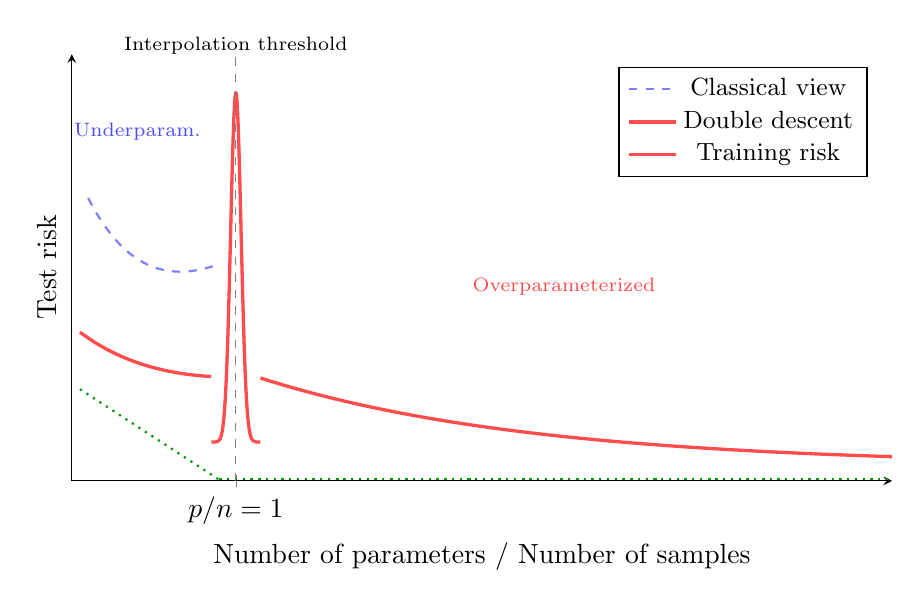
\begin{tikzpicture}[scale=1.0]
    \begin{axis}[
        width=12cm, height=7cm,
        xlabel={Number of parameters / Number of samples},
        ylabel={Test risk},
        xmin=0, xmax=5,
        ymin=0, ymax=2.2,
        xtick={1},
        xticklabels={$p/n = 1$},
        ytick=\empty,
        axis lines=left,
        domain=0:5,
        samples=200,
        clip=false,
        legend style={at={(0.97,0.97)}, anchor=north east, font=\small},
    ]
        % Classical U-shaped curve (bias-variance)
        \addplot[blue!50, thick, dashed, domain=0.1:0.9] {1.5*exp(-2*x) + 0.8*x + 0.15};
        \addlegendentry{Classical view}

        % Double descent curve
        \addplot[red!70, very thick, domain=0.05:0.85] {0.6*exp(-1.5*x) + 0.2*x + 0.2};
        \addplot[red!70, very thick, domain=0.85:1.15] {0.2 + 1.8*exp(-50*(x-1)^2/(0.1))};
        \addplot[red!70, very thick, domain=1.15:5] {0.45*exp(-0.6*(x-1.15)) + 0.08};
        \addlegendentry{Double descent}

        % Training risk
        \addplot[green!60!black, thick, dotted, domain=0.05:0.9] {max(0.5 - 0.55*x, 0.01)};
        \addplot[green!60!black, thick, dotted, domain=0.9:5] {0.01};
        \addlegendentry{Training risk}

        % Vertical line at interpolation threshold
        \draw[gray, dashed, thin] (axis cs:1, 0) -- (axis cs:1, 2.2);
        \node[above, font=\scriptsize] at (axis cs:1, 2.15) {Interpolation threshold};

        % Region labels
        \node[font=\scriptsize, blue!70] at (axis cs:0.4, 1.8) {Underparam.};
        \node[font=\scriptsize, red!70] at (axis cs:3, 1.0) {Overparameterized};
    \end{axis}
\end{tikzpicture}
\caption{Double descent curve: the test risk decreases again
in the overparameterized regime, contradicting the classical bias-variance trade-off.}
\label{fig:double-descent}
\end{figure}

\subsection{Implicit Bias of Gradient Descent}

\begin{theorem}[Implicit Bias --- Linear Regression]
\label{thm:implicit-bias}
For overparameterized linear regression ($p > n$), gradient
descent initialized at $\mathbf{w}_0 = \mathbf{0}$ converges to
the minimum-norm solution:
\begin{equation}
\mathbf{w}^* = \argmin_{\mathbf{w}} \|\mathbf{w}\| \quad \text{s.t.} \quad \mathbf{X}\mathbf{w} = \mathbf{y}
\end{equation}
\end{theorem}

\begin{proof}
Gradient descent produces $\mathbf{w}_t \in \text{Im}(\mathbf{X}^\top)$
at each iteration. The interpolator in this space is unique and
corresponds to the pseudo-inverse solution $\mathbf{w}^* = \mathbf{X}^\top(\mathbf{X}\mathbf{X}^\top)^{-1}\mathbf{y}$,
which is of minimum norm by construction.
\end{proof}

\begin{remark}
For nonlinear networks, the implicit bias is more complex
and depends on the architecture, the learning rate, and the batch
size. See also Chapter~\ref{ch:backpropagation} for
connections with SGD.
\end{remark}

% ============================================================
\section{Neural Tangent Kernel (NTK)}
\label{sec:ntk}
\index{NTK}\index{neural tangent kernel}

\subsection{Linearization at Initialization}

\begin{definition}[Neural Tangent Kernel]
\label{def:ntk}
Let $f(\mathbf{x}; \boldsymbol{\theta})$ be a neural network. The NTK
is defined by:
\begin{equation}
\Theta(\mathbf{x}, \mathbf{x}') = \left\langle \frac{\partial f(\mathbf{x}; \boldsymbol{\theta})}{\partial \boldsymbol{\theta}},\, \frac{\partial f(\mathbf{x}'; \boldsymbol{\theta})}{\partial \boldsymbol{\theta}} \right\rangle = \sum_{i=1}^{P} \frac{\partial f(\mathbf{x}; \boldsymbol{\theta})}{\partial \theta_i} \frac{\partial f(\mathbf{x}'; \boldsymbol{\theta})}{\partial \theta_i}
\end{equation}
where $P$ is the total number of parameters.
\end{definition}

\begin{theorem}[NTK Convergence --- Jacot et al., 2018]
\label{thm:ntk-convergence}
For a network with $L$ layers of width $n_\ell \to \infty$ with
NTK parameterization, the kernel $\Theta(\mathbf{x}, \mathbf{x}')$
converges in probability to a deterministic kernel $\Theta^*(\mathbf{x}, \mathbf{x}')$
at initialization, and \emph{remains constant} during training.
\end{theorem}

\subsection{Derivation of the Linearization}

\begin{mathbox}[title=\textbf{Taylor Linearization of the Network}]
In the neighborhood of the initialization $\boldsymbol{\theta}_0$:
\begin{equation}
f(\mathbf{x}; \boldsymbol{\theta}) \approx f(\mathbf{x}; \boldsymbol{\theta}_0) + \nabla_{\boldsymbol{\theta}} f(\mathbf{x}; \boldsymbol{\theta}_0)^\top (\boldsymbol{\theta} - \boldsymbol{\theta}_0)
\end{equation}
Under this approximation, training by gradient descent on the
quadratic loss yields:
\begin{equation}
\frac{d\mathbf{f}}{dt} = -\eta\,\boldsymbol{\Theta}_0\,(\mathbf{f}(t) - \mathbf{y})
\end{equation}
where $\mathbf{f}(t) = (f(x_1; \boldsymbol{\theta}_t), \ldots, f(x_n; \boldsymbol{\theta}_t))^\top$
and $[\boldsymbol{\Theta}_0]_{ij} = \Theta(\mathbf{x}_i, \mathbf{x}_j)\big|_{\boldsymbol{\theta}_0}$.

The solution is:
\begin{equation}
\mathbf{f}(t) = \mathbf{y} - e^{-\eta\,\boldsymbol{\Theta}_0\,t}(\mathbf{y} - \mathbf{f}(0))
\end{equation}
which shows exponential convergence to interpolation $\mathbf{f} = \mathbf{y}$
if $\boldsymbol{\Theta}_0 \succ 0$.
\end{mathbox}

\begin{remark}
NTK theory explains training in the so-called ``lazy'' regime
(small weight variation). In practice, networks often operate
in a ``rich'' regime where representations evolve
significantly.
\end{remark}

% ============================================================
\section{Expressivity: Depth vs Width}
\label{sec:expressivity}
\index{expressivity}

\subsection{Universal Approximation Theorem}

\begin{theorem}[Cybenko, 1989; Hornik, 1991]
\label{thm:universal-approx}
A one-hidden-layer network with continuous non-polynomial activation
can approximate any continuous function on a compact set to arbitrary
precision $\varepsilon$, provided the width is sufficient.
\end{theorem}

\begin{warning}
This theorem is an \emph{existence} result: it says nothing about
the required width, which can be exponentially large.
\end{warning}

\subsection{Depth-Width Separation}

\begin{theorem}[Telgarsky, 2016]
\label{thm:depth-separation}
There exist functions computable by a ReLU network of depth $L$
and width $O(1)$ that require width $\Omega(2^{L/3})$ to be
approximated by a network of depth $O(1)$.
\end{theorem}

\begin{proof}[Sketch]
Consider the ``sawtooth'' function $g : [0,1] \to [0,1]$
defined by $g(x) = 2\min(x, 1-x)$. The iterated composition
$g^{\circ k} = g \circ \cdots \circ g$ ($k$ times) is a piecewise
linear function with $2^k$ pieces. Now:
\begin{itemize}
    \item $g^{\circ k}$ is realizable by a ReLU network of depth $2k$
          and width $2$: $g(x) = \relu(2x) - 2\relu(2x - 1)$.
    \item A network of depth $\ell$ and width $w$ produces at most
          $O(w^\ell)$ linear regions.
\end{itemize}
If $\ell$ is constant, one needs $w = \Omega(2^{k/\ell})$ regions,
hence the exponential separation.
\end{proof}

% ============================================================
\section{Lottery Ticket Hypothesis}
\label{sec:lottery-ticket}
\index{lottery ticket hypothesis}

\begin{theorem}[Frankle \& Carlin, 2019 --- Lottery Ticket Hypothesis]
\label{thm:lottery}
A randomly initialized dense network contains a subnetwork
(\emph{winning ticket}) that, when trained in isolation with the same initial
weights, achieves comparable performance to the full network in a
comparable number of iterations.
\end{theorem}

\begin{remark}
Identifying the winning subnetwork is done through iterative magnitude
pruning: train, prune the lowest-magnitude weights,
reset to the original weights, and repeat.
Compression rates reach $90$--$99\%$ on certain architectures.
\end{remark}

% ============================================================
\section{Geometry of the Loss Landscape}
\label{sec:loss-landscape}
\index{loss landscape}\index{SAM}

\subsection{Saddle Points and Flat Minima}

\begin{proposition}[Predominance of Saddle Points]
\label{prop:saddle-points}
In a high-dimensional space of dimension $d$, critical points
(where $\nabla L = 0$) are exponentially more likely to be
saddle points than local minima. If each eigenvalue of the
Hessian is positive or negative with probability $1/2$, the probability
of a local minimum is $2^{-d}$.
\end{proposition}

\begin{definition}[Sharpness-Aware Minimization (SAM)]
\label{def:sam}
SAM seeks parameters in ``flat'' regions by optimizing:
\begin{equation}
\min_{\boldsymbol{\theta}} \max_{\|\boldsymbol{\epsilon}\| \leq \rho} L(\boldsymbol{\theta} + \boldsymbol{\epsilon})
\end{equation}
The first-order approximation yields the update:
\begin{equation}
\hat{\boldsymbol{\epsilon}} = \rho \frac{\nabla_{\boldsymbol{\theta}} L(\boldsymbol{\theta})}{\|\nabla_{\boldsymbol{\theta}} L(\boldsymbol{\theta})\|}, \quad
\boldsymbol{\theta} \leftarrow \boldsymbol{\theta} - \eta\,\nabla_{\boldsymbol{\theta}} L(\boldsymbol{\theta} + \hat{\boldsymbol{\epsilon}})
\end{equation}
\end{definition}

\begin{figure}[htbp]
\centering
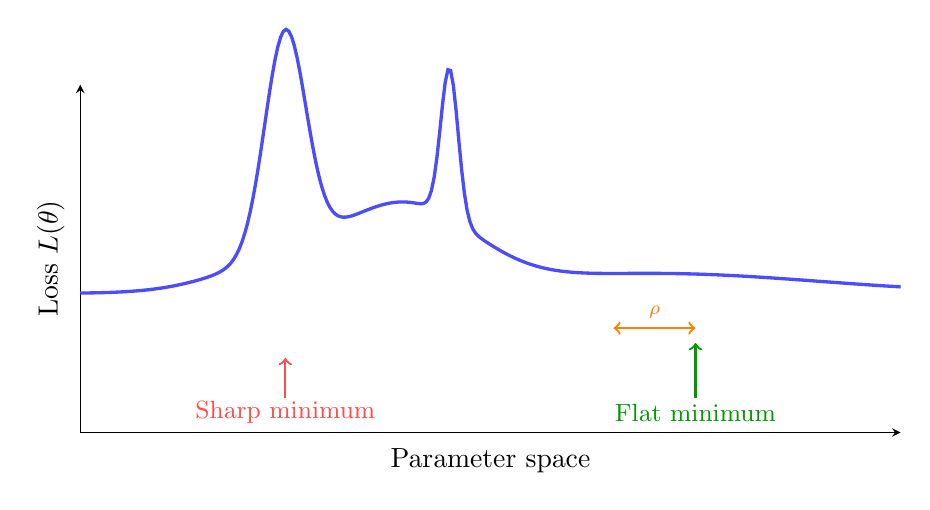
\begin{tikzpicture}[scale=1.0]
    \begin{axis}[
        width=12cm, height=6cm,
        xlabel={Parameter space},
        ylabel={Loss $L(\boldsymbol{\theta})$},
        xmin=-4, xmax=6,
        ymin=-0.5, ymax=3,
        xtick=\empty, ytick=\empty,
        axis lines=left,
        domain=-4:6,
        samples=300,
        clip=false,
    ]
        % Sharp minimum
        \addplot[blue!70, very thick] {
            0.3 + 2.2*exp(-0.5*((x+1.5)/0.25)^2)*(x > -2.5)*(x < -0.5) +
            0.3*exp(-0.5*((x+1.5)/0.8)^2) +
            0.6 + 1.5*exp(-((x-0.5)/0.15)^2) +
            0.2*exp(-0.5*((x-3)/2)^2) +
            0.8*exp(-0.5*((x)/0.8)^2)
        };

        % Annotations
        \node[font=\small, red!70] at (axis cs:-1.5, -0.3) {Sharp minimum};
        \draw[->, red!70, thick] (axis cs:-1.5, -0.15) -- (axis cs:-1.5, 0.25);

        \node[font=\small, green!60!black] at (axis cs:3.5, -0.3) {Flat minimum};
        \draw[->, green!60!black, thick] (axis cs:3.5, -0.15) -- (axis cs:3.5, 0.4);

        % Epsilon ball illustration
        \draw[<->, orange, thick] (axis cs:2.5, 0.55) -- node[above, font=\scriptsize] {$\rho$} (axis cs:3.5, 0.55);
    \end{axis}
\end{tikzpicture}
\caption{Sharp vs flat minima: SAM favors flat minima that
generalize better because the loss varies little within a neighborhood of radius $\rho$.}
\label{fig:sharp-flat-minima}
\end{figure}

% ============================================================
\section{Information Bottleneck Theory}
\label{sec:information-bottleneck}
\index{information bottleneck}

\begin{definition}[Bottleneck Principle]
\label{def:info-bottleneck}
Let $X$ be the input, $Y$ the target, and $T$ the internal representation.
The IB principle seeks to:
\begin{equation}
\min_{p(t|x)} \; I(X; T) - \beta\,I(T; Y)
\end{equation}
where $I(\cdot;\cdot)$ denotes mutual information and $\beta > 0$
controls the compression/prediction trade-off.
\end{definition}

\begin{remark}
Shwartz-Ziv \& Tishby (2017) conjecture that training of deep
networks goes through two phases: (1) \emph{fitting} where $I(T;Y)$ increases,
then (2) \emph{compression} where $I(X;T)$ decreases. This theory remains
debated: the results depend on the activation function and
the mutual information estimator used.
\end{remark}

% ============================================================
\section{Experimental Demonstration of Double Descent}
\label{sec:double-descent-exp}

\begin{codeblock}[title=\textbf{Experimental double descent with variable-width networks}]
\begin{minted}{python}
import torch
import torch.nn as nn
import numpy as np
from sklearn.datasets import make_classification
from sklearn.model_selection import train_test_split

# Data: binary classification, small n to observe double descent
X, y = make_classification(n_samples=200, n_features=20,
                           n_informative=10, random_state=42)
X_train, X_test, y_train, y_test = train_test_split(
    X, y, test_size=0.3, random_state=42)

X_train_t = torch.tensor(X_train, dtype=torch.float32)
y_train_t = torch.tensor(y_train, dtype=torch.float32).unsqueeze(1)
X_test_t = torch.tensor(X_test, dtype=torch.float32)
y_test_t = torch.tensor(y_test, dtype=torch.float32).unsqueeze(1)

def make_model(width):
    return nn.Sequential(
        nn.Linear(20, width), nn.ReLU(),
        nn.Linear(width, width), nn.ReLU(),
        nn.Linear(width, 1))

def train_and_eval(width, epochs=2000, lr=1e-3):
    model = make_model(width)
    opt = torch.optim.Adam(model.parameters(), lr=lr)
    loss_fn = nn.BCEWithLogitsLoss()
    for _ in range(epochs):
        opt.zero_grad()
        loss_fn(model(X_train_t), y_train_t).backward()
        opt.step()
    with torch.no_grad():
        train_loss = loss_fn(model(X_train_t), y_train_t).item()
        test_loss = loss_fn(model(X_test_t), y_test_t).item()
    return train_loss, test_loss

# Vary the width (number of parameters)
widths = [2, 4, 6, 8, 10, 15, 20, 30, 50, 80, 120, 200, 400, 800]
results = []
for w in widths:
    n_params = 20*w + w + w*w + w + w*1 + 1  # count the parameters
    tr, te = train_and_eval(w)
    results.append((w, n_params, tr, te))
    print(f"Width={w:4d}, Params={n_params:6d}, "
          f"Train={tr:.4f}, Test={te:.4f}")
\end{minted}
\end{codeblock}

\begin{codeoutput}
\begin{verbatim}
Width=   2, Params=     49, Train=0.5814, Test=0.6231
Width=   4, Params=     97, Train=0.4012, Test=0.4893
Width=  10, Params=    331, Train=0.1254, Test=0.3891
Width=  20, Params=    861, Train=0.0312, Test=0.5127
Width=  30, Params=   1591, Train=0.0041, Test=0.4203
Width=  50, Params=   3851, Train=0.0003, Test=0.3542
Width= 120, Params=  17161, Train=0.0001, Test=0.3201
Width= 400, Params= 168801, Train=0.0001, Test=0.2987
Width= 800, Params= 657601, Train=0.0001, Test=0.2854
\end{verbatim}
\end{codeoutput}

\begin{remark}
We observe that the test risk first increases (around $w = 20$,
near the interpolation threshold), then decreases in the
overparameterized regime. This behavior illustrates double descent.
\end{remark}

% ============================================================
\section{State of the Art and Recent Connections}
\label{sec:theory-sota}

\begin{sota}[title=\textbf{Deep Learning Theory in 2024--2025}]
\begin{itemize}
    \item \textbf{Grokking}\index{grokking}: phenomenon where a model
          first memorizes the training data, then
          ``understands'' the underlying structure after a very
          large number of epochs, going from zero generalization
          to perfect generalization. Partially explained by
          the implicit regularization of \emph{weight decay}.
    \item \textbf{Neural scaling laws}\index{scaling laws}:
          Kaplan et al.\ (2020) and Hoffmann et al.\ (2022, ``Chinchilla'')
          show that the loss follows power laws:
          \begin{equation}
          L(N, D) \approx \left(\frac{N_c}{N}\right)^{\alpha_N} + \left(\frac{D_c}{D}\right)^{\alpha_D} + L_\infty
          \end{equation}
          where $N$ is the number of parameters and $D$ the data size.
    \item \textbf{Mechanistic interpretability}\index{mechanistic interpretability}:
          analysis of the internal circuits of networks to understand
          \emph{how} they implement algorithms. Examples:
          induction circuits in Transformers, feature superposition.
    \item \textbf{Feature learning vs kernel regime}: distinction between
          the NTK regime (``lazy'', no representation learning)
          and the rich regime (``feature learning''), the latter being
          the one observed in practice.
\end{itemize}
\end{sota}

% ============================================================
\section{Exercises}
\label{sec:theory-exercises}

\begin{exercise}[VC Dimension \textmd{($\star$)}]
\label{exo:vc-dim}
Show that the VC dimension of linear classifiers in $\R^2$
is $3$ by exhibiting a shatterable set of $3$ points and by
showing that no set of $4$ points can be shattered.
\end{exercise}

\begin{exercise}[Rademacher Complexity \textmd{($\star\star$)}]
\label{exo:rademacher}
Let $\mathcal{H} = \{x \mapsto \mathbf{w}^\top x : \|\mathbf{w}\| \leq B\}$.
Show that:
\begin{equation}
\hat{\mathfrak{R}}_S(\mathcal{H}) \leq \frac{B\sqrt{\sum_{i=1}^{m}\|x_i\|^2}}{m}
\end{equation}
\textit{Hint: use the Cauchy-Schwarz inequality.}
\end{exercise}

\begin{exercise}[NTK for a One-Layer Network \textmd{($\star\star$)}]
\label{exo:ntk-one-layer}
Consider $f(\mathbf{x}; \boldsymbol{\theta}) = \frac{1}{\sqrt{n}}\sum_{j=1}^{n} a_j\,\sigma(\mathbf{w}_j^\top \mathbf{x})$
where $\sigma = \relu$, $a_j \sim \mathcal{N}(0, 1)$ fixed, and
$\mathbf{w}_j \sim \mathcal{N}(\mathbf{0}, \mathbf{I})$.
\begin{enumerate}
    \item Compute $\Theta(\mathbf{x}, \mathbf{x}') = \sum_j \frac{\partial f}{\partial \mathbf{w}_j} \cdot \frac{\partial f}{\partial \mathbf{w}_j}$ explicitly.
    \item Show that as $n \to \infty$, $\Theta(\mathbf{x}, \mathbf{x}')$ converges to a deterministic kernel.
    \item Express this kernel as a function of the angle between $\mathbf{x}$ and $\mathbf{x}'$.
\end{enumerate}
\end{exercise}

\begin{exercise}[Depth-Width Separation \textmd{($\star\star\star$)}]
\label{exo:depth-separation}
Let $g(x) = 2\min(x, 1-x)$ for $x \in [0,1]$.
\begin{enumerate}
    \item Show that $g$ can be written as a ReLU network of depth
          $2$ and width $2$.
    \item Show that $g^{\circ k}$ has $2^k$ linear pieces.
    \item Deduce that a network of depth $\ell$ and width $w$
          cannot represent $g^{\circ k}$ if $w^\ell < 2^k$.
\end{enumerate}
\end{exercise}

\begin{exercise}[Implicit Bias of SGD \textmd{($\star\star$)}]
\label{exo:implicit-bias}
In the overparameterized linear regression setting:
\begin{enumerate}
    \item Prove that gradient descent with $\mathbf{w}_0 = \mathbf{0}$
          maintains $\mathbf{w}_t \in \text{Im}(\mathbf{X}^\top)$ for all $t$.
    \item Show that the unique interpolator in $\text{Im}(\mathbf{X}^\top)$
          is $\mathbf{X}^\dagger \mathbf{y}$ (pseudo-inverse).
    \item Discuss how this result sheds light on the generalization
          of overparameterized networks.
\end{enumerate}
\end{exercise}

\begin{exercise}[Experimental SAM \textmd{($\star\star$)}]
\label{exo:sam}
\begin{enumerate}
    \item Implement the SAM optimizer in PyTorch (two gradient passes
          per iteration).
    \item Compare SGD, Adam and SAM on CIFAR-10 with a ResNet-18.
    \item Measure the ``sharpness'' of the found minimum (largest
          eigenvalue of the Hessian, approximated by the power method).
    \item Verify that SAM finds flatter minima and generalizes better.
\end{enumerate}
\end{exercise}

\begin{exercise}[Scaling Laws \textmd{($\star$)}]
\label{exo:scaling-laws}
Language models of sizes $N \in \{10^6, 10^7, 10^8, 10^9\}$
parameters are trained and test losses $L \in \{3.2, 2.8, 2.5, 2.3\}$ are observed.
\begin{enumerate}
    \item Plot $\log L$ as a function of $\log N$.
    \item Estimate the exponent $\alpha_N$ by linear regression.
    \item Extrapolate the loss for $N = 10^{11}$.
    \item Discuss the limitations of this extrapolation.
\end{enumerate}
\end{exercise}
